\documentclass{article} % For LaTex2e
\usepackage{iclr2022_conference,times}
% Optional math commands from https://github.com/goodfeli/dlbook_notation.
%%%%% NEW MATH DEFINITIONS %%%%%

\usepackage{amsmath,amsfonts,bm}

% Mark sections of captions for referring to divisions of figures
\newcommand{\figleft}{{\em (Left)}}
\newcommand{\figcenter}{{\em (Center)}}
\newcommand{\figright}{{\em (Right)}}
\newcommand{\figtop}{{\em (Top)}}
\newcommand{\figbottom}{{\em (Bottom)}}
\newcommand{\captiona}{{\em (a)}}
\newcommand{\captionb}{{\em (b)}}
\newcommand{\captionc}{{\em (c)}}
\newcommand{\captiond}{{\em (d)}}

% Highlight a newly defined term
\newcommand{\newterm}[1]{{\bf #1}}


% Figure reference, lower-case.
\def\figref#1{figure~\ref{#1}}
% Figure reference, capital. For start of sentence
\def\Figref#1{Figure~\ref{#1}}
\def\twofigref#1#2{figures \ref{#1} and \ref{#2}}
\def\quadfigref#1#2#3#4{figures \ref{#1}, \ref{#2}, \ref{#3} and \ref{#4}}
% Section reference, lower-case.
\def\secref#1{section~\ref{#1}}
% Section reference, capital.
\def\Secref#1{Section~\ref{#1}}
% Reference to two sections.
\def\twosecrefs#1#2{sections \ref{#1} and \ref{#2}}
% Reference to three sections.
\def\secrefs#1#2#3{sections \ref{#1}, \ref{#2} and \ref{#3}}
% Reference to an equation, lower-case.
\def\eqref#1{equation~\ref{#1}}
% Reference to an equation, upper case
\def\Eqref#1{Equation~\ref{#1}}
% A raw reference to an equation---avoid using if possible
\def\plaineqref#1{\ref{#1}}
% Reference to a chapter, lower-case.
\def\chapref#1{chapter~\ref{#1}}
% Reference to an equation, upper case.
\def\Chapref#1{Chapter~\ref{#1}}
% Reference to a range of chapters
\def\rangechapref#1#2{chapters\ref{#1}--\ref{#2}}
% Reference to an algorithm, lower-case.
\def\algref#1{algorithm~\ref{#1}}
% Reference to an algorithm, upper case.
\def\Algref#1{Algorithm~\ref{#1}}
\def\twoalgref#1#2{algorithms \ref{#1} and \ref{#2}}
\def\Twoalgref#1#2{Algorithms \ref{#1} and \ref{#2}}
% Reference to a part, lower case
\def\partref#1{part~\ref{#1}}
% Reference to a part, upper case
\def\Partref#1{Part~\ref{#1}}
\def\twopartref#1#2{parts \ref{#1} and \ref{#2}}

\def\ceil#1{\lceil #1 \rceil}
\def\floor#1{\lfloor #1 \rfloor}
\def\1{\bm{1}}
\newcommand{\train}{\mathcal{D}}
\newcommand{\valid}{\mathcal{D_{\mathrm{valid}}}}
\newcommand{\test}{\mathcal{D_{\mathrm{test}}}}

\def\eps{{\epsilon}}


% Random variables
\def\reta{{\textnormal{$\eta$}}}
\def\ra{{\textnormal{a}}}
\def\rb{{\textnormal{b}}}
\def\rc{{\textnormal{c}}}
\def\rd{{\textnormal{d}}}
\def\re{{\textnormal{e}}}
\def\rf{{\textnormal{f}}}
\def\rg{{\textnormal{g}}}
\def\rh{{\textnormal{h}}}
\def\ri{{\textnormal{i}}}
\def\rj{{\textnormal{j}}}
\def\rk{{\textnormal{k}}}
\def\rl{{\textnormal{l}}}
% rm is already a command, just don't name any random variables m
\def\rn{{\textnormal{n}}}
\def\ro{{\textnormal{o}}}
\def\rp{{\textnormal{p}}}
\def\rq{{\textnormal{q}}}
\def\rr{{\textnormal{r}}}
\def\rs{{\textnormal{s}}}
\def\rt{{\textnormal{t}}}
\def\ru{{\textnormal{u}}}
\def\rv{{\textnormal{v}}}
\def\rw{{\textnormal{w}}}
\def\rx{{\textnormal{x}}}
\def\ry{{\textnormal{y}}}
\def\rz{{\textnormal{z}}}

% Random vectors
\def\rvepsilon{{\mathbf{\epsilon}}}
\def\rvtheta{{\mathbf{\theta}}}
\def\rva{{\mathbf{a}}}
\def\rvb{{\mathbf{b}}}
\def\rvc{{\mathbf{c}}}
\def\rvd{{\mathbf{d}}}
\def\rve{{\mathbf{e}}}
\def\rvf{{\mathbf{f}}}
\def\rvg{{\mathbf{g}}}
\def\rvh{{\mathbf{h}}}
\def\rvu{{\mathbf{i}}}
\def\rvj{{\mathbf{j}}}
\def\rvk{{\mathbf{k}}}
\def\rvl{{\mathbf{l}}}
\def\rvm{{\mathbf{m}}}
\def\rvn{{\mathbf{n}}}
\def\rvo{{\mathbf{o}}}
\def\rvp{{\mathbf{p}}}
\def\rvq{{\mathbf{q}}}
\def\rvr{{\mathbf{r}}}
\def\rvs{{\mathbf{s}}}
\def\rvt{{\mathbf{t}}}
\def\rvu{{\mathbf{u}}}
\def\rvv{{\mathbf{v}}}
\def\rvw{{\mathbf{w}}}
\def\rvx{{\mathbf{x}}}
\def\rvy{{\mathbf{y}}}
\def\rvz{{\mathbf{z}}}

% Elements of random vectors
\def\erva{{\textnormal{a}}}
\def\ervb{{\textnormal{b}}}
\def\ervc{{\textnormal{c}}}
\def\ervd{{\textnormal{d}}}
\def\erve{{\textnormal{e}}}
\def\ervf{{\textnormal{f}}}
\def\ervg{{\textnormal{g}}}
\def\ervh{{\textnormal{h}}}
\def\ervi{{\textnormal{i}}}
\def\ervj{{\textnormal{j}}}
\def\ervk{{\textnormal{k}}}
\def\ervl{{\textnormal{l}}}
\def\ervm{{\textnormal{m}}}
\def\ervn{{\textnormal{n}}}
\def\ervo{{\textnormal{o}}}
\def\ervp{{\textnormal{p}}}
\def\ervq{{\textnormal{q}}}
\def\ervr{{\textnormal{r}}}
\def\ervs{{\textnormal{s}}}
\def\ervt{{\textnormal{t}}}
\def\ervu{{\textnormal{u}}}
\def\ervv{{\textnormal{v}}}
\def\ervw{{\textnormal{w}}}
\def\ervx{{\textnormal{x}}}
\def\ervy{{\textnormal{y}}}
\def\ervz{{\textnormal{z}}}

% Random matrices
\def\rmA{{\mathbf{A}}}
\def\rmB{{\mathbf{B}}}
\def\rmC{{\mathbf{C}}}
\def\rmD{{\mathbf{D}}}
\def\rmE{{\mathbf{E}}}
\def\rmF{{\mathbf{F}}}
\def\rmG{{\mathbf{G}}}
\def\rmH{{\mathbf{H}}}
\def\rmI{{\mathbf{I}}}
\def\rmJ{{\mathbf{J}}}
\def\rmK{{\mathbf{K}}}
\def\rmL{{\mathbf{L}}}
\def\rmM{{\mathbf{M}}}
\def\rmN{{\mathbf{N}}}
\def\rmO{{\mathbf{O}}}
\def\rmP{{\mathbf{P}}}
\def\rmQ{{\mathbf{Q}}}
\def\rmR{{\mathbf{R}}}
\def\rmS{{\mathbf{S}}}
\def\rmT{{\mathbf{T}}}
\def\rmU{{\mathbf{U}}}
\def\rmV{{\mathbf{V}}}
\def\rmW{{\mathbf{W}}}
\def\rmX{{\mathbf{X}}}
\def\rmY{{\mathbf{Y}}}
\def\rmZ{{\mathbf{Z}}}

% Elements of random matrices
\def\ermA{{\textnormal{A}}}
\def\ermB{{\textnormal{B}}}
\def\ermC{{\textnormal{C}}}
\def\ermD{{\textnormal{D}}}
\def\ermE{{\textnormal{E}}}
\def\ermF{{\textnormal{F}}}
\def\ermG{{\textnormal{G}}}
\def\ermH{{\textnormal{H}}}
\def\ermI{{\textnormal{I}}}
\def\ermJ{{\textnormal{J}}}
\def\ermK{{\textnormal{K}}}
\def\ermL{{\textnormal{L}}}
\def\ermM{{\textnormal{M}}}
\def\ermN{{\textnormal{N}}}
\def\ermO{{\textnormal{O}}}
\def\ermP{{\textnormal{P}}}
\def\ermQ{{\textnormal{Q}}}
\def\ermR{{\textnormal{R}}}
\def\ermS{{\textnormal{S}}}
\def\ermT{{\textnormal{T}}}
\def\ermU{{\textnormal{U}}}
\def\ermV{{\textnormal{V}}}
\def\ermW{{\textnormal{W}}}
\def\ermX{{\textnormal{X}}}
\def\ermY{{\textnormal{Y}}}
\def\ermZ{{\textnormal{Z}}}

% Vectors
\def\vzero{{\bm{0}}}
\def\vone{{\bm{1}}}
\def\vmu{{\bm{\mu}}}
\def\vtheta{{\bm{\theta}}}
\def\va{{\bm{a}}}
\def\vb{{\bm{b}}}
\def\vc{{\bm{c}}}
\def\vd{{\bm{d}}}
\def\ve{{\bm{e}}}
\def\vf{{\bm{f}}}
\def\vg{{\bm{g}}}
\def\vh{{\bm{h}}}
\def\vi{{\bm{i}}}
\def\vj{{\bm{j}}}
\def\vk{{\bm{k}}}
\def\vl{{\bm{l}}}
\def\vm{{\bm{m}}}
\def\vn{{\bm{n}}}
\def\vo{{\bm{o}}}
\def\vp{{\bm{p}}}
\def\vq{{\bm{q}}}
\def\vr{{\bm{r}}}
\def\vs{{\bm{s}}}
\def\vt{{\bm{t}}}
\def\vu{{\bm{u}}}
\def\vv{{\bm{v}}}
\def\vw{{\bm{w}}}
\def\vx{{\bm{x}}}
\def\vy{{\bm{y}}}
\def\vz{{\bm{z}}}

% Elements of vectors
\def\evalpha{{\alpha}}
\def\evbeta{{\beta}}
\def\evepsilon{{\epsilon}}
\def\evlambda{{\lambda}}
\def\evomega{{\omega}}
\def\evmu{{\mu}}
\def\evpsi{{\psi}}
\def\evsigma{{\sigma}}
\def\evtheta{{\theta}}
\def\eva{{a}}
\def\evb{{b}}
\def\evc{{c}}
\def\evd{{d}}
\def\eve{{e}}
\def\evf{{f}}
\def\evg{{g}}
\def\evh{{h}}
\def\evi{{i}}
\def\evj{{j}}
\def\evk{{k}}
\def\evl{{l}}
\def\evm{{m}}
\def\evn{{n}}
\def\evo{{o}}
\def\evp{{p}}
\def\evq{{q}}
\def\evr{{r}}
\def\evs{{s}}
\def\evt{{t}}
\def\evu{{u}}
\def\evv{{v}}
\def\evw{{w}}
\def\evx{{x}}
\def\evy{{y}}
\def\evz{{z}}

% Matrix
\def\mA{{\bm{A}}}
\def\mB{{\bm{B}}}
\def\mC{{\bm{C}}}
\def\mD{{\bm{D}}}
\def\mE{{\bm{E}}}
\def\mF{{\bm{F}}}
\def\mG{{\bm{G}}}
\def\mH{{\bm{H}}}
\def\mI{{\bm{I}}}
\def\mJ{{\bm{J}}}
\def\mK{{\bm{K}}}
\def\mL{{\bm{L}}}
\def\mM{{\bm{M}}}
\def\mN{{\bm{N}}}
\def\mO{{\bm{O}}}
\def\mP{{\bm{P}}}
\def\mQ{{\bm{Q}}}
\def\mR{{\bm{R}}}
\def\mS{{\bm{S}}}
\def\mT{{\bm{T}}}
\def\mU{{\bm{U}}}
\def\mV{{\bm{V}}}
\def\mW{{\bm{W}}}
\def\mX{{\bm{X}}}
\def\mY{{\bm{Y}}}
\def\mZ{{\bm{Z}}}
\def\mBeta{{\bm{\beta}}}
\def\mPhi{{\bm{\Phi}}}
\def\mLambda{{\bm{\Lambda}}}
\def\mSigma{{\bm{\Sigma}}}

% Tensor
\DeclareMathAlphabet{\mathsfit}{\encodingdefault}{\sfdefault}{m}{sl}
\SetMathAlphabet{\mathsfit}{bold}{\encodingdefault}{\sfdefault}{bx}{n}
\newcommand{\tens}[1]{\bm{\mathsfit{#1}}}
\def\tA{{\tens{A}}}
\def\tB{{\tens{B}}}
\def\tC{{\tens{C}}}
\def\tD{{\tens{D}}}
\def\tE{{\tens{E}}}
\def\tF{{\tens{F}}}
\def\tG{{\tens{G}}}
\def\tH{{\tens{H}}}
\def\tI{{\tens{I}}}
\def\tJ{{\tens{J}}}
\def\tK{{\tens{K}}}
\def\tL{{\tens{L}}}
\def\tM{{\tens{M}}}
\def\tN{{\tens{N}}}
\def\tO{{\tens{O}}}
\def\tP{{\tens{P}}}
\def\tQ{{\tens{Q}}}
\def\tR{{\tens{R}}}
\def\tS{{\tens{S}}}
\def\tT{{\tens{T}}}
\def\tU{{\tens{U}}}
\def\tV{{\tens{V}}}
\def\tW{{\tens{W}}}
\def\tX{{\tens{X}}}
\def\tY{{\tens{Y}}}
\def\tZ{{\tens{Z}}}


% Graph
\def\gA{{\mathcal{A}}}
\def\gB{{\mathcal{B}}}
\def\gC{{\mathcal{C}}}
\def\gD{{\mathcal{D}}}
\def\gE{{\mathcal{E}}}
\def\gF{{\mathcal{F}}}
\def\gG{{\mathcal{G}}}
\def\gH{{\mathcal{H}}}
\def\gI{{\mathcal{I}}}
\def\gJ{{\mathcal{J}}}
\def\gK{{\mathcal{K}}}
\def\gL{{\mathcal{L}}}
\def\gM{{\mathcal{M}}}
\def\gN{{\mathcal{N}}}
\def\gO{{\mathcal{O}}}
\def\gP{{\mathcal{P}}}
\def\gQ{{\mathcal{Q}}}
\def\gR{{\mathcal{R}}}
\def\gS{{\mathcal{S}}}
\def\gT{{\mathcal{T}}}
\def\gU{{\mathcal{U}}}
\def\gV{{\mathcal{V}}}
\def\gW{{\mathcal{W}}}
\def\gX{{\mathcal{X}}}
\def\gY{{\mathcal{Y}}}
\def\gZ{{\mathcal{Z}}}

% Sets
\def\sA{{\mathbb{A}}}
\def\sB{{\mathbb{B}}}
\def\sC{{\mathbb{C}}}
\def\sD{{\mathbb{D}}}
% Don't use a set called E, because this would be the same as our symbol
% for expectation.
\def\sF{{\mathbb{F}}}
\def\sG{{\mathbb{G}}}
\def\sH{{\mathbb{H}}}
\def\sI{{\mathbb{I}}}
\def\sJ{{\mathbb{J}}}
\def\sK{{\mathbb{K}}}
\def\sL{{\mathbb{L}}}
\def\sM{{\mathbb{M}}}
\def\sN{{\mathbb{N}}}
\def\sO{{\mathbb{O}}}
\def\sP{{\mathbb{P}}}
\def\sQ{{\mathbb{Q}}}
\def\sR{{\mathbb{R}}}
\def\sS{{\mathbb{S}}}
\def\sT{{\mathbb{T}}}
\def\sU{{\mathbb{U}}}
\def\sV{{\mathbb{V}}}
\def\sW{{\mathbb{W}}}
\def\sX{{\mathbb{X}}}
\def\sY{{\mathbb{Y}}}
\def\sZ{{\mathbb{Z}}}

% Entries of a matrix
\def\emLambda{{\Lambda}}
\def\emA{{A}}
\def\emB{{B}}
\def\emC{{C}}
\def\emD{{D}}
\def\emE{{E}}
\def\emF{{F}}
\def\emG{{G}}
\def\emH{{H}}
\def\emI{{I}}
\def\emJ{{J}}
\def\emK{{K}}
\def\emL{{L}}
\def\emM{{M}}
\def\emN{{N}}
\def\emO{{O}}
\def\emP{{P}}
\def\emQ{{Q}}
\def\emR{{R}}
\def\emS{{S}}
\def\emT{{T}}
\def\emU{{U}}
\def\emV{{V}}
\def\emW{{W}}
\def\emX{{X}}
\def\emY{{Y}}
\def\emZ{{Z}}
\def\emSigma{{\Sigma}}

% entries of a tensor
% Same font as tensor, without \bm wrapper
\newcommand{\etens}[1]{\mathsfit{#1}}
\def\etLambda{{\etens{\Lambda}}}
\def\etA{{\etens{A}}}
\def\etB{{\etens{B}}}
\def\etC{{\etens{C}}}
\def\etD{{\etens{D}}}
\def\etE{{\etens{E}}}
\def\etF{{\etens{F}}}
\def\etG{{\etens{G}}}
\def\etH{{\etens{H}}}
\def\etI{{\etens{I}}}
\def\etJ{{\etens{J}}}
\def\etK{{\etens{K}}}
\def\etL{{\etens{L}}}
\def\etM{{\etens{M}}}
\def\etN{{\etens{N}}}
\def\etO{{\etens{O}}}
\def\etP{{\etens{P}}}
\def\etQ{{\etens{Q}}}
\def\etR{{\etens{R}}}
\def\etS{{\etens{S}}}
\def\etT{{\etens{T}}}
\def\etU{{\etens{U}}}
\def\etV{{\etens{V}}}
\def\etW{{\etens{W}}}
\def\etX{{\etens{X}}}
\def\etY{{\etens{Y}}}
\def\etZ{{\etens{Z}}}

% The true underlying data generating distribution
\newcommand{\pdata}{p_{\rm{data}}}
% The empirical distribution defined by the training set
\newcommand{\ptrain}{\hat{p}_{\rm{data}}}
\newcommand{\Ptrain}{\hat{P}_{\rm{data}}}
% The model distribution
\newcommand{\pmodel}{p_{\rm{model}}}
\newcommand{\Pmodel}{P_{\rm{model}}}
\newcommand{\ptildemodel}{\tilde{p}_{\rm{model}}}
% Stochastic autoencoder distributions
\newcommand{\pencode}{p_{\rm{encoder}}}
\newcommand{\pdecode}{p_{\rm{decoder}}}
\newcommand{\precons}{p_{\rm{reconstruct}}}

\newcommand{\laplace}{\mathrm{Laplace}} % Laplace distribution

\newcommand{\E}{\mathbb{E}}
\newcommand{\Ls}{\mathcal{L}}
\newcommand{\R}{\mathbb{R}}
\newcommand{\emp}{\tilde{p}}
\newcommand{\lr}{\alpha}
\newcommand{\reg}{\lambda}
\newcommand{\rect}{\mathrm{rectifier}}
\newcommand{\softmax}{\mathrm{softmax}}
\newcommand{\sigmoid}{\sigma}
\newcommand{\softplus}{\zeta}
\newcommand{\KL}{D_{\mathrm{KL}}}
\newcommand{\Var}{\mathrm{Var}}
\newcommand{\standarderror}{\mathrm{SE}}
\newcommand{\Cov}{\mathrm{Cov}}
% Wolfram Mathworld says $L^2$ is for function spaces and $\ell^2$ is for vectors
% But then they seem to use $L^2$ for vectors throughout the site, and so does
% wikipedia.
\newcommand{\normlzero}{L^0}
\newcommand{\normlone}{L^1}
\newcommand{\normltwo}{L^2}
\newcommand{\normlp}{L^p}
\newcommand{\normmax}{L^\infty}

\newcommand{\parents}{Pa} % See usage in notation.tex. Chosen to match Daphne's book.

\DeclareMathOperator*{\argmax}{arg\,max}
\DeclareMathOperator*{\argmin}{arg\,min}

\DeclareMathOperator{\sign}{sign}
\DeclareMathOperator{\Tr}{Tr}
\let\ab\allowbreak


%######## MAT292: Uncomment your submission name
\newcommand{\matname}{ - Group 1 Project Proposal}
%\newcommand{\matname}{Progress Report}
%\newcommand{\matname}{Final Report}

%######## MAT292: Put your Group Number here
%\newcommand{\gpnumber}{40}

\usepackage{hyperref}
\usepackage{xcolor}
\usepackage[normalem]{ulem}
\usepackage{url}
\usepackage{graphicx}
\usepackage{placeins}
\usepackage{float}
\usepackage{tikz}
\usepackage{multicol, breqn}
\usepackage{caption}

%######## MAT292: Put your project Title here
\title{Real-Time Neural Signal Filtering via \\
Hodgkin-Huxley Simulation Models}

%######## MAT292: Put your names, student IDs and Emails here
\author{\textbf{Peter Leong} \\
    Student\# 1010892955 \\
    peter.leong@mail.utoronto.ca
\And
    \textbf{Karys Littlejohns} \\
    Student\# 1010893142 \\
    karys.littlejohns@mail.utoronto.ca
\And
    \textbf{Katherine Shepherd} \\
    Student\# 1010895097 \\
    k.shepherd@mail.utoronto.ca
}



\iclrfinalcopy 
%######## MAT292: Document starts here
\begin{document}

\maketitle

% add vertical space between authors and abstract
%\vspace{2ex}   % <-- adjust this value as needed


% \begin{abstract}

% %######## MAT292: Do not change the next line. This shows your Main body page count.
% ----Total Pages: \pageref{last_page}
% \end{abstract}

\vspace{2ex}

\begin{multicols}{2}

\section{Introduction}
\label{sec:introduction}
Spike detection from noisy extracellular recordings is crucial for advancing brain-computer interfaces and neuroscience research. 
Neural action potentials are well-modeled by the Hodgkin-Huxley (H-H) equations, which describe the ionic conductance changes underlying these waveforms. 
Our work adapts H-H generated waveforms to simulate realistic noisy conditions.

Beyond EEG and microelectrode arrays, neural signal processing enables critical applications including epileptic seizure prediction \citep{addai-domfe2024epileptic} and adaptive deep brain stimulation for Parkinson's disease \citep{aljalal2022parkinson}. 
The emergence of high-density neural probes further motivates efficient filtering solutions for handling large data streams \citep{ye2024ultra}. 

The primary goal of this project is to develop and validate a spike detection algorithm that operates accurately in low signal-to-noise ratio environments by leveraging synthetic data generated from the H-H model.

\section{Scope \& Feasibility}
\label{sec:scope_feasibility}

This project applies concepts from ESC103: Engineering Mathematics \& Computation and MAT292: Ordinary Differential Equations through four sequential, feasible phases:
(1) generating synthetic neural data by solving the Hodgkin-Huxley equations,
(2) processing this data with a digital filter,
(3) developing a spike detection algorithm, and
(4) quantitative comparison using Peak-Signal-to-Noise Ratio and local truncation error analysis.
The phased approach and inclusion of buffer time make this scope achievable within the 12-week timeline.

\subsection{Project Objectives}
\label{subsec:project_objectives}

\textbf{Data Generation:} Implement numerical solvers for the Hodgkin-Huxley model to generate realistic synthetic action potential data.

\textbf{Signal Processing:} Design and apply a digital band-pass filter to isolate spike waveforms from generated signals with added synthetic noise.

\textbf{Spike Detection:} Develop an algorithm that detects action potentials using an adaptive threshold based on the estimated noise floor.

\textbf{Validation:} Qualitatively and quantitatively assess detection algorithm performance on noisy synthetic data.

\subsection{Project Milestones \& Timeline}
\label{subsec:milestones_timeline}

Key milestones from our detailed Gantt chart (\ref{app:a_gantt_chart}) ensure steady progress toward our objectives: \textbf{Week 4:} Complete Euler's and Improved Euler's method solvers and first noise generation algorithm.
\textbf{Week 6:} Implement Runge-Kutta method solver(s) and first band-pass filter iteration.
\textbf{Week 8:} Refine all components: band-pass filter, noise generation, and numerical methods.
\textbf{Week 10:} Final results evaluation and report completion.
\textbf{Weeks 11-12:} Buffer time for unexpected delays.
\section{Technical Background}
\label{sec:technical_background}

Understanding neuronal biology is essential for appreciating the abstractions in the Hodgkin-Huxley equations. 
This section covers the fundamentals of neural action potentials, the underlying biochemical processes, key equations from the H-H model, and the numerical methods used in our analysis.

\subsection{The Biological Basis: Ion Channels and Currents}
\label{subsec:biological_basis}

Electrophysiology—the study of electrical properties of cells—provides the basis for cell communication via current signals. 
This supports not only the neural signalling process, but also fundamental processes like muscle contraction, nutrient transport, and cellular homeostasis. 
These current signals work tangentially with ion channels—pores discovered by Hodgkin and Huxley that use selective permeability to regulate intramolecular transport across lipid bilayers. 
Ion channels occur when current flows across a cell membrane. This transport occurs bi-directionally, its flux reversing as the Nernst potential is reached (zero-current state). 
Ion channel movement can be measured via the ionic currents that pass through, this measurement is based on Ohm's Law \citep{rubaiy2017electrophysiology}.

\subsection{The Cell Membrane and Electric Potentials}
\label{subsubsec:resting_potential}

Action potential is the change in membrane electric potential that creates ion channels \cite{rubaiy2017electrophysiology}. 
The cell electrical state is measured as $V_{m}$, the potential difference between the cytoplasm and external environment \cite{cervera2016bioelectrical}. 
In their resting state, cell membranes possess a net negative charge (resting potential), preventing ion channel creation. 
Depolarization occurs when a membrane changes from a net negative charge to a net positive charge, opening an ion channel. 
Repolarization occurs when the membrane regains its negative charge, closing the ion channel \cite{rubaiy2017electrophysiology}. 
This electrical bi-stability of depolarization to repolarization is an important characteristic of neural cells \cite{cervera2016bioelectrical}.

\subsection{Hodgkin-Huxley Equations}
\label{subsec:hodgekin_huxley}

The Hodgkin-Huxley model is a system of nonlinear differential equations that represent action potentials movement through nerve cells by three types of ion current: sodium, potassium, and a leak current. 
Describing the transfer of these ions with a circuit allows for equations that model cells electrical properties \cite{Schwiening2012}. 

\subsubsection{Model Components and Equations}
\label{subsubsec:hh_equations}
\begin{minipage}{\linewidth}
    \centering
    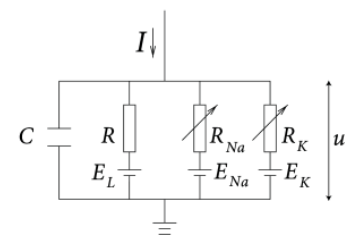
\includegraphics[width=0.9\linewidth]{Figs/ion_circuit.png}
    \captionof{figure}{Circuit representation of ion transfer across the cell membrane \cite{Gerstner2014}}
    \label{fig:ion_circuit}
\end{minipage}
The circuit model represents each component of ion transfer within a nerve cell as an electrical component: 
the ion pumps and the leak channel are represented as resistors; the difference in ion concentration for each ion is represented by a battery; the lipid bilayer is represented by a capacitor \cite{Gerstner2014}.
These components are combined according to the circuit in Figure~\ref{fig:ion_circuit}, to create the equation for current across the cell membrane:
\begin{dmath}
    I = C_{M}\frac{dV}{dt} + \bar{g}_{K}n^4(V - V_{K}) + \bar{g}_{Na}m^3h(V - V_{Na}) + \bar{g}_{l}(V - V_{l})
    \label{eq:ion_current}
\end{dmath}
Relating Equation~\ref{eq:ion_current} to Figure~\ref{fig:ion_circuit}, V is analogous to u, and $V_x$ to $E_x$ (where x represents Na, K, or l). Discerned from the resistance values, $g_x$ (where x is Na, K, or l) represents the maximum conductance of the channel.

\subsubsection{Gating Variables and Activation/Inactivation}
\label{subsubsec:gating_variables}

Hodgkins and Huxley theorized that specific ammounts of charged particles would need to move under influence of the membrane potential to allow $Na^+$ or $K^+$ particles to move \cite{Schwiening2012}.
Based on this theory, the model uses three gating variables (m, n, and h) to represent the probability that a channel will be open at a given moment in time. 
For the $Na^+$ channels, m describes the activation of the channel and h is its inactivation. 
Similarly, n describes the activation of the $K^+$ channels.
They found that $n^4$, $m^3$, and h provided a good fit \cite{Schwiening2012}. 
The gating variables are represented across a range of potentials by equations of the form:
\begin{dmath}
    \dot{x} = -\frac{1}{\tau_{x}(u)}[x - x_{0}(u)]
    \label{eq:gating_variables}
\end{dmath}
To interpret Equation~\ref{eq:gating_variables}, let $\dot{x}$ = $\frac{dx}{dt}$ where x stands for m, n, or h. $\tau_0$(u) and $x_0$(u) are conditional variables dependent on the initial membrane potential \cite{Gerstner2014}.

\subsection{Numerical Methods}
\label{subsec:numerical_methods}

Many real-world differential equations do not possess elegant algebraic solutions; however, this does not prevent us from understanding their solutions. 
Numerical methods offer a powerful alternative, enabling us to visualize and approximate solutions with considerable accuracy. 
Our work focuses on three foundational techniques: Euler's Method, Improved Euler's Method, and the Runge-Kutta Method. 
We detail Euler's Method in this section, while comprehensive explanations of the others are available in \ref{app:c_numerical_methods}. 
All derivations and governing equations are sourced from \cite{brannan2015differential}.

\subsubsection{Euler's Method}
\label{subsubsec:euler_method}

Intuitively, Euler's Method solves the initial value problem by constructing an approximate solution from connected tangent line segments over discrete time intervals. 
Given a differential equation with initial condition:
\[
    \frac{dy}{dt} = f(t, y) \quad \text{with} \quad y(t_0) = y_0
\]
we begin at the initial point $(t_0, y_0)$ and use the slope given by $f(t_0, y_0)$ to construct the first tangent line:
\[
    y = y_0 + f(t_0, y_0)(t - t_0)
\]
This linear approximation provides our next point $(t_1, y_1)$ by evaluating at $t = t_1$. We then iterate this process, using each new point $(t_n, y_n)$ to compute the next approximation:
\[
    y_{n+1} = y_n + f(t_n, y_n) \cdot \Delta t
\]
where $\Delta t = t_{n+1} - t_n$ is the fixed step size. 
As the number of steps increases and $\Delta t$ decreases, this piecewise linear approximation converges toward the true solution curve $\phi(t)$.

\label{last_page}

\newpage
\bibliographystyle{iclr2022_conference}
\bibliography{MAT292_Proposal_Ref}

\end{multicols}

\newpage
\appendix

\section{Gantt Chart}
\label{app:a_gantt_chart}
\begin{figure}[htbp]
  \centering
  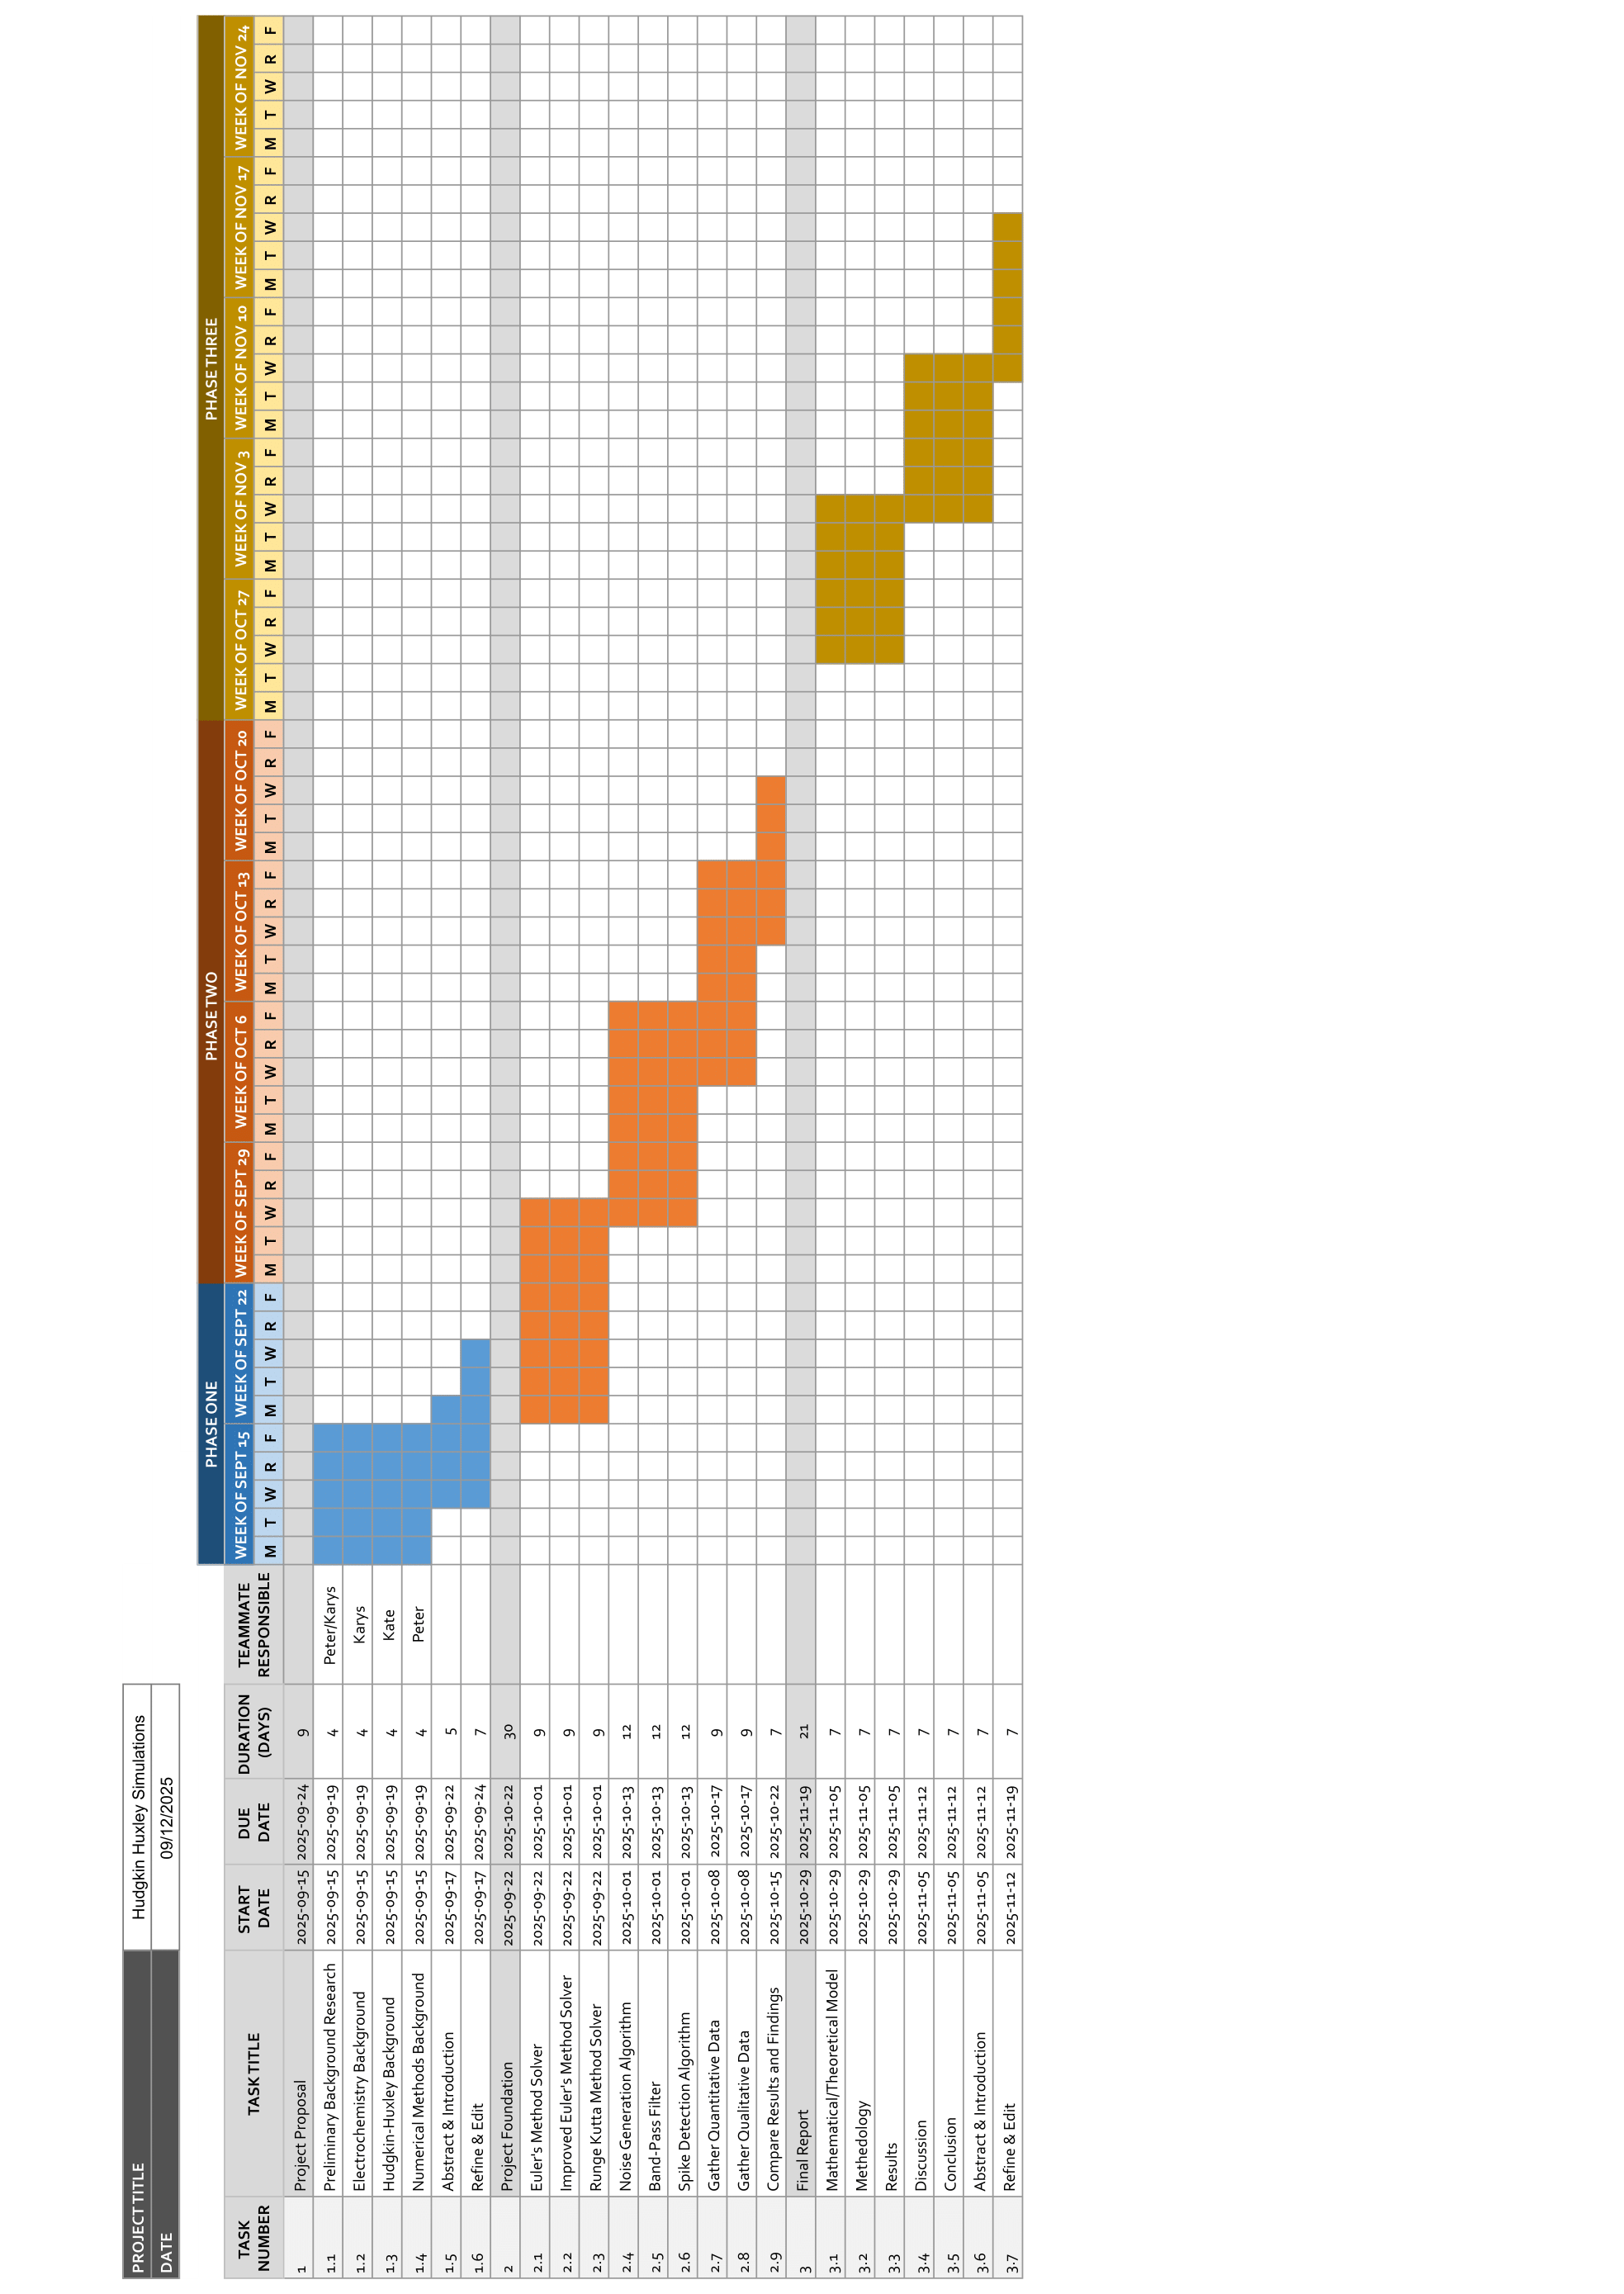
\includegraphics[width=0.88\linewidth]{Figs/gantt_chart_rot.png}
    \caption{Our project plan is organized into three distinct phases with integrated buffers between them.
            Direct access to the chart can be found \href{https://docs.google.com/spreadsheets/d/1jHzTcHqw4nSWZ5ZlPa9hzeYbwHf0eZ49koE-SQ0onvM/edit?usp=sharing}{here}}
\end{figure}

\end{document}
